\documentclass[12pt]{article}
\usepackage{alltt}
\usepackage[utf8]{inputenc}
\usepackage[dvips]{graphicx}
%\usepackage{a4wide}
\usepackage{epsfig}
\usepackage{fancybox}
\usepackage{verbatim}
\usepackage{array}
\usepackage{latexsym}
\usepackage{alltt}
%\usepackage{dsfont}
\usepackage{caption}
\usepackage{subcaption}
%\usepackage{fullpage}
\usepackage{hyperref}
\usepackage{textcomp}
\usepackage{listings}
\usepackage{color}
\usepackage{amsmath}
\usepackage{amsfonts}
\usepackage{tikz}
\usepackage{float}
\usepackage{matlab-prettifier}
\usepackage{graphicx}

\usepackage[hmargin=3cm,vmargin=6.0cm]{geometry}
%\topmargin=0cm
\topmargin=-2cm
\addtolength{\textheight}{6.5cm}
\addtolength{\textwidth}{2.0cm}
%\setlength{\leftmargin}{-5cm}
\setlength{\oddsidemargin}{0.0cm}
\setlength{\evensidemargin}{0.0cm}

%misc libraries goes here

\begin{document}

\section*{Student Information } 
%Write your full name and id number between the colon and newline
%Put one empty space character after colon and before newline
Full Name : Doruk Berke Yurtsizoglu \\
Id Number :  2522225\\

% Write your answers below the section tags
\section*{Answer 1}

\subsection*{a)} 
The time taken to process and send the response is uniformly distributed which means the density is constant. The pdf of uniform distribution is:\\
$\dfrac{1}{b-a}$, for $a \leq t \leq b$\\
\\
Since A and B are independent, we can find the joint density function ($f(t_A , t_B )$) by simply taking the product of $f(t_A)$ and $f(t_B)$.\\
$f(t_A , t_B )$ = $f(t_A)$ *  $f(t_B)$ \\
$f(t_A , t_B )$ = $\dfrac{1}{100}$ * $\dfrac{1}{100}$ = 0.0001\\
\\
We can find the e joint cdf like finding the joint pdf. Take the product of $F(t_A)$ and $F(t_B)$.\\
Joint cdf is the integral taken version of joint pdf. In this case our separate cdf's will be in the form of:\\
\\
$\dfrac{x}{b-a}$, for $a \leq x \leq b$\\
 So, $F(t_A , t_B )$ = $F(t_A)$ *  $F(t_B)$ = $\dfrac{t_A}{100}$ * $\dfrac{t_B}{100}$ = $\dfrac{t_A * t_B}{10000}$\\


\subsection*{b)} 

We will use the joint cdf function to find the probabilities.\\
$-$ For the probability that server A processes the packet and sends a response within the first 30 milliseconds:\\
\\
$P(0 \leq t_A \leq 30)$ = $\dfrac{30 - 0}{100}$ = 0.3\\
\\
$-$ For the probability that  server B takes between 40 and 60 milliseconds to process the packet and send a response:\\
\\
$P(40 \leq t_A \leq 60)$ = $\dfrac{60 - 40}{100}$ = 0.2\\
\\
Since these events are independent, in order to find the probability that server A processes the packet and sends a response within the first
30 milliseconds, while server B takes between 40 and 60 milliseconds to process the packet and send a response, we simply need to take the product of the probabilities that we have found which is equal to 0.3 * 0.2 = 0.06.\\


\subsection*{c)} 

The realition between $T_A$ and $T_B$ is $T_A - T_B \leq 10$. Than the probability that we want to find is:\\
$P(T_A - T_B \leq 10)$ = $\iint f(t_A , t_B ) dt_A \ dt_B $\\
\\
In order to take the integral correctly, we need to separate the interval to 2 parts.\\
$-$ While $0 \leq t_B \leq 90$ then $0 \leq t_A \leq t_B + 10$\\
$-$ While $90 < t_B \leq 100$ then $0 \leq t_A \leq 100$\\
\\
After this step, our equation looks like:\\
$P(T_A - T_B \leq 10)$ = $\int_{0}^{90} \int_{0}^{T_B + 10} f(t_A , t_B ) dt_A \ dt_B $ + $\int_{90}^{100} \int_{0}^{100} f(t_A , t_B ) dt_A \ dt_B $\\
\\
The result of this equation is $\dfrac{99}{200}$ * $\dfrac{10}{100}$ = $\dfrac{119}{200}$ \\


\subsection*{d)} 
The realition between $T_A$ and $T_B$ is $|T_A - T_B| \leq 20$. Than the probability that we want to find is:\\
$P(|T_A - T_B| \leq 20)$ = $\iint f(t_A , t_B ) dt_A \ dt_B $\\
\\
This time in order to take the integral correctly, we need to separate the interval to 3 parts.\\
$-$ While $20 \leq t_B \leq 80$ then $t_B - 20 \leq t_A \leq t_B + 20$\\
$-$ While $0 \leq t_B < 20$ then $0 \leq t_A \leq t_B + 20$\\
$-$ While $80 \leq t_B < 100$ then $t_B - 20 \leq t_A \leq t_B + 100$\\
\\
After this step, our equation looks like:\\
$P(|T_A - T_B| \leq 20)$ =  $\int_{20}^{80} \int_{T_B - 20}^{T_B + 20} f(t_A , t_B ) dt_A \ dt_B $ +  $\int_{0}^{20} \int_{0}^{T_B + 20} f(t_A , t_B ) dt_A \ dt_B $ + \\  $\int_{80}^{100} \int_{T_B - 20}^{100} f(t_A , t_B ) dt_A \ dt_B $\\
\\
$P(|T_A - T_B| \leq 20)$ = $\dfrac{6}{25}$ + $\dfrac{3}{50}$ + $\dfrac{3}{50}$ = $\dfrac{9}{25}$ = 0.36\\


\section*{Answer 2}

\subsection*{a)} 
The question is a normal approximation to binomial because we know that p = 0.6, n = 150 and q = 0.4.  Each Bernoulli Trial in this binomial distribution question has a mean which is equal to 0.6 and a standard deviation which is $\sqrt{p * q}$ = 0.49.\\
So, $\mu$ = 0.6 and $\sigma$ = 0.49 for each Bernoulli Trial.\\
\\
Since $n \geq 30$ we can use normal approximation.\\
The probability that is asked changes to:\\
 $P(X > 0.65) \rightarrow = P(S_n \geq 0.65*150) = P(S_n \geq 97.5) = P(S_n > 97)$.\\
We must apply continuity correction in order to approximate appropriately. (Which is $P(S_n \geq 97.5)$ for continuous case.)\\

$P(S_n \geq 97.5)$ = $P(\dfrac{S_n - n*\mu}{\sigma * \sqrt{n}} \geq \dfrac{97.5 - 150*0.6}{0.49*\sqrt{150}})$

Then $P(S_n \geq 97.5)$ = $P(Z > 1.25)$ = 1 - $\Phi (1.25)$ = 1 - 0.8944 = 0.1056\\

\subsection*{b)} 

This question is same as the previous one. This time p = 0.1(mean), and standard deviation =  $\sqrt{p * q}$ = 0.3\\
So, $\mu$ = 0.1 and $\sigma$ = 0.3 for each Bernoulli Trial.\\
\\
Since $n \geq 30$ we can use normal approximation.\\
The probability that is asked changes to:\\
 $P(X > 0.65) \rightarrow = P(S_n \leq 0.15*150) = P(S_n \leq 22.5) = P(S_n < 23)$.\\
We must apply continuity correction in order to approximate appropriately. (Which is $P(S_n \leq 22.5)$ for continuous case.)\\

$P(S_n \leq 22.5)$ = $P(\dfrac{S_n - n*\mu}{\sigma * \sqrt{n}} \leq \dfrac{22.5 - 150*0.1}{0.3*\sqrt{150}})$

Then $P(S_n \leq 22.5)$ = $P(Z < 2.04)$ = = $\Phi (2.04)$ = 0.9793\\

\section*{Answer 3}
The question is $P(170 \leq X \leq 180)$\\
The mean $(\mu)$ is 175.\\
The standard deviation $(\sigma)$ is 7.\\
\\
We are going to standardize both 170, X and 180.\\
Standardizing formula = $z = \dfrac{x - \mu}{\sigma}$\\
\\
Let's standardize 170, X and 180.\\
$-$ X $\rightarrow z$\\
$-$ 170 $\rightarrow \dfrac{170 - 175}{7}$ = -0.71\\
\\
$-$ 180 $\rightarrow \dfrac{180 - 175}{7}$ = 0.71\\
\\
Then $P(170 \leq X \leq 180)$ = $P(-0.71 \leq z \leq 0.71)$ = $\Phi (0.71)$ - (1 - $\Phi (0.71))$ = 0.5222\\


\section*{Answer 4}

\subsection*{a)} 
\begin{lstlisting}[style=Matlab-editor]

%% My Code
part_a()

function [] = part_a()
    mean = 175;
    std_deviation = 7;
    N = 1000;
    heights_db = normrnd(mean, std_deviation, N, 1);
    
    figure
    histogram(heights_db);
    xlabel('Height (cm)', 'FontSize', 11);
    ylabel('Amount of people', 'FontSize', 11);
    title('Distribution of Heights')
end

\end{lstlisting}

\begin{figure}[H]
  \centering
  \begin{subfigure}[b]{0.4\linewidth}
    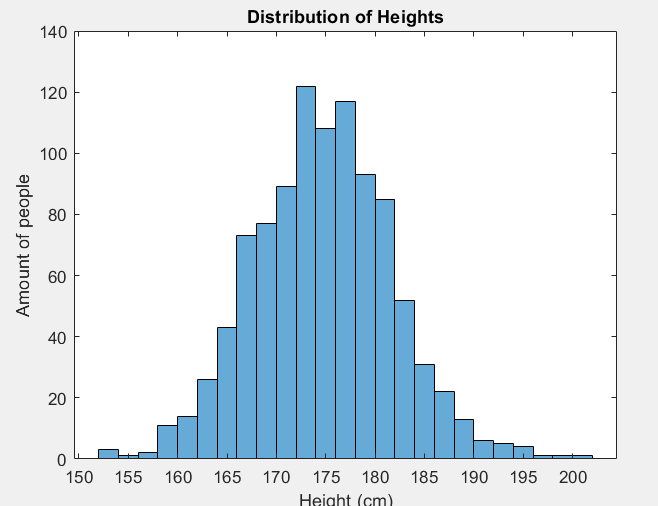
\includegraphics[width=\linewidth]{Screenshot (1458).png}
    \caption{Since the mean is 175 cm, the distribution of heights gathered around 175 cm on the histogram.}
  \end{subfigure}
\end{figure}

\subsection*{b)} 
\begin{lstlisting}[style=Matlab-editor]

%% My Code
part_b()

function [] = part_b()
    x = linspace(130, 220, 1000);
    mean = 175;
    pdf6 = normpdf(x, mean, 6);
    pdf7 = normpdf(x, mean, 7);
    pdf8 = normpdf(x, mean, 8);
    
    figure
    plot(x, pdf6, 'LineWidth', 1.5)
    hold on
    plot(x, pdf7, 'LineWidth', 1.5)
    plot(x, pdf8, 'LineWidth', 1.5)
    xlabel('Height (cm)', 'FontSize', 11)
    ylabel('Probability Density', 'FontSize', 11)
    title('PDF for Different Values of Standard Deviation', 'FontSize', 11);
    legend('\sigma = 6', '\sigma = 7', '\sigma = 8')
end

\end{lstlisting}

\begin{figure}[H]
  \centering
  \begin{subfigure}[b]{0.4\linewidth}
    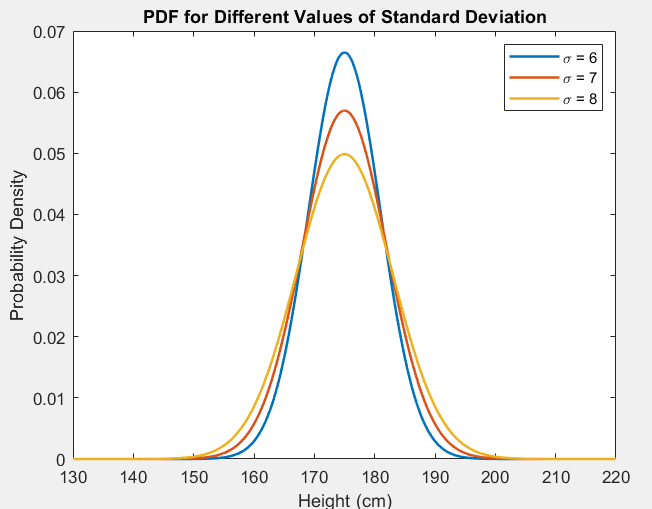
\includegraphics[width=\linewidth]{Screenshot (1459).png}
    \caption{As the standard deviation increases, we observe that the distribution becomes sharper around the mean since std.deviation is as known as scale parameter too.}
  \end{subfigure}
\end{figure}


\subsection*{c)} 
\begin{lstlisting}[style=Matlab-editor]

%% My Code
part_c()

function [] = part_c()
    % Define variables
    mean = 175;
    std_dev = 7;
    sample_size = 150;
    
    l_bound = 170;
    u_bound = 180;
    
    N = 1000;
    proportion_vec = [0.45, 0.50, 0.55];
    num_props = length(proportion_vec);
    success_counts = zeros(1, num_props);
    
    % Simulate experiments
    for i = 1:N
        sample_data = normrnd(mean, std_dev, sample_size, 1);
        
        % Check how many samples lie within the bounds
        num_within_bounds = sum(sample_data > l_bound & sample_data < u_bound);
        
        % Check if proportion of samples within bounds exceeds threshold
        for j = 1:num_props
            if num_within_bounds / sample_size >= proportion_vec(j)
                success_counts(j) = success_counts(j) + 1;
            end
        end
    end
    
    % Compute probabilities and print results
    success_probs = success_counts / N;
    for j = 1:num_props
        disp(['Probability of at least %' num2str(proportion_vec(j)*100) ' of adults with heights between 170 and 180: ' num2str(success_probs(j))]);
    end
end
\end{lstlisting}


\begin{figure}[H]
  \centering
  \begin{subfigure}[b]{0.4\linewidth}
    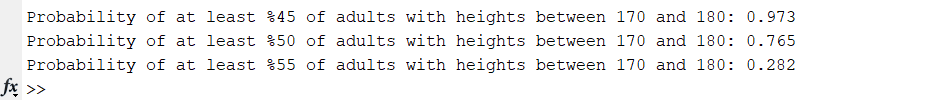
\includegraphics[width=\linewidth]{Screenshot (1461).png}
    \caption{We observe that, as the proportion of samples in [170cm,180cm] becomes greater, the probability decreases dramatically.}
  \end{subfigure}
\end{figure}
\end{document}